\documentclass[conference]{IEEEtran}
\IEEEoverridecommandlockouts
% The preceding line is only needed to identify funding in the first footnote. If that is unneeded, please comment it out.
\usepackage{cite}
\usepackage{amsmath,amssymb,amsfonts}
\usepackage{algorithmic}
\usepackage{graphicx}
\usepackage{textcomp}
\usepackage{xcolor}
\def\BibTeX{{\rm B\kern-.05em{\sc i\kern-.025em b}\kern-.08em
    T\kern-.1667em\lower.7ex\hbox{E}\kern-.125emX}}
\begin{document}

\title{A Survey of Security Issues in Federated Laearning}

\author{\IEEEauthorblockN{1\textsuperscript{st} Yunhao Feng}
    \IEEEauthorblockA{\textit{National University of Defense and Technology} \\
        Changsha, China \\
        fengyunhaonudt@nudt.edu.cn}
    \and
    \IEEEauthorblockN{2\textsuperscript{nd} Yinjian Hou}
    \IEEEauthorblockA{\textit{National University of Defense and Technology} \\
        Changsha, China \\
        houyinjian18@nudt.edu.cn}

}

\maketitle

\begin{abstract}
    As people's awareness of the importance of personal privacy protection has grown,
    there has been a surge of interest in federated learning,
    which is a machine learning paradigm that enables training without requiring
    access to users' private data.
\end{abstract}



\section{Introduction}
The rapid development of digital technology has made the diversification, informationization,
and diversity of digital data the main topics of the current era. Meanwhile, deep learning (DL) has
demonstrated tremendous success in multiple fields, including computer vision, natural language
processing, and graphic networks. Clearly, using diverse data in deep learning models can effectively
improve their ability. However, there is also a growing interest in data privacy protection,
such as the General Data Protection Regulation (GDPR)\cite{b1}. On the other hand, data sources may
encounter the challenge of distributed storage, as is the case with data from mobile smart devices
or Internet of Things (IoT) scenarios\cite{b2},\cite{b3}. Therefore, utilizing these data to train models requires
overcoming limitations related to distribution and privacy\cite{b4}.

To solve these problems, federated learning(FL) is a machine learning paradigm proposed as a possible response to these
challenges\cite{b5}. FL enables collaborative model building among distributed members while ensuring sensitive data remains
within each participant's control\cite{b6}. Specifically, federated learning allows two or more participants to collaboratively
train a shared global DL model while keeping their training datasets locally. Each participant trains the shared model on its own
training data and exchanges and updates model parameters with other participants. Federated learning can improve the training speed
and the performance of the shared model while protecting privacy of the participants' training datasets\cite{b7}. Thus, it is a promising
technique for the scenarios where the training data is sensitive (e.g., medical records, personally identifiable information, etc.) \cite{b8},\cite{b9}.

\begin{figure}[htbp]
    \centerline{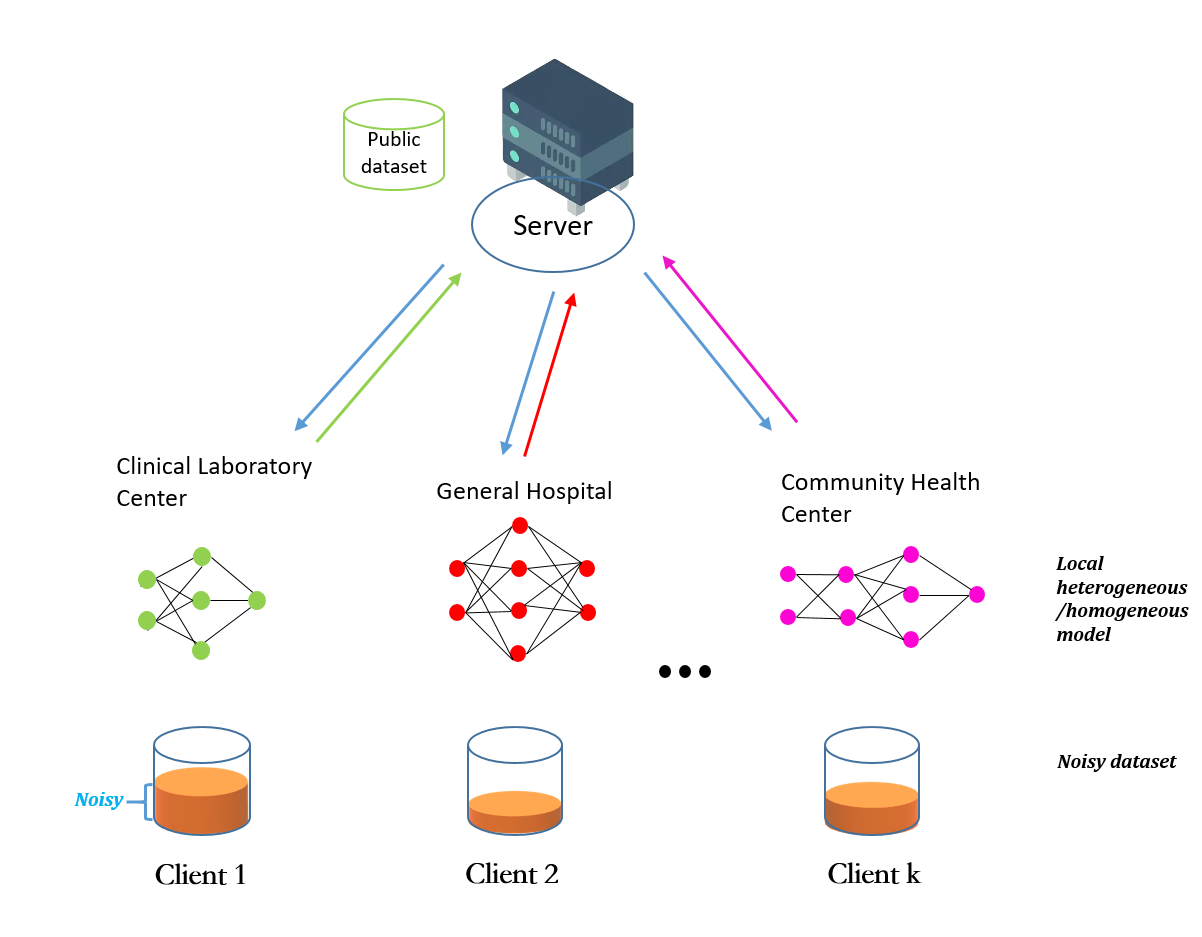
\includegraphics[width=0.8\linewidth,height=0.4\linewidth]{picture/f1.png}}
    \caption{A schematic of federated learning.}
    \label{fig1}
\end{figure}

Federated learning can be classified based on whether the participating datasets are the same, resulting in two types: homogeneous federated
learning  and heterogeneous federated learning \cite{b10},\cite{b11}. In homogeneous federated
learning, all participants have datasets with the same characteristics and data distribution, whereas in heterogeneous federated learning,
participants' datasets may differ in their characteristics and data distribution. The second classification of federated learning is based
on whether the models involved are the same, resulting in two types: horizontal federated learning and vertical
federated learning\cite{b12},\cite{b13}. In horizontal federated learning, all participants have the same model architecture, but may
have different local data\cite{b14}, while in vertical federated learning, each participant has a different model architecture but they collaborate on
processing the same set of data together\cite{b15}. The third way to classify federated learning is based on the type of task involved, resulting in several
types such as federated learning for clustering\cite{b16},\cite{b17}, federated learning for classification\cite{b18},\cite{b19}, federated learning for regression\cite{b20}, among others.
The fourth way to classify federated learning is based on the optimization approach used between the participants, resulting in several types such as
federated averaging\cite{b21},\cite{b22}, federated learning optimization, federated meta-learning\cite{b23}, and so on.

Federated learning methods currently face significant challenges related to their robustness. This article focuses on three main attacks. including backdoor attacks\cite{b24},\cite{b25},\cite{b26},\cite{b27},\cite{b28}, adversarial attacks\cite{b31},\cite{b32},\cite{b33},\cite{b34}, and Byzantine attacks\cite{b29},\cite{b30}.
A backdoor attack involves a malicious participant in the federated learning process adding a backdoor to the model being trained, which can be triggered by a specific input pattern,
allowing the attacker to control the output of the model in a targeted way. Adversarial attacks, on the other hand, entail adding small,
carefully crafted perturbations to the input data to deceive the model and cause it to make incorrect predictions\cite{b31},\cite{b32}.

\begin{figure}[htbp]
    \centerline{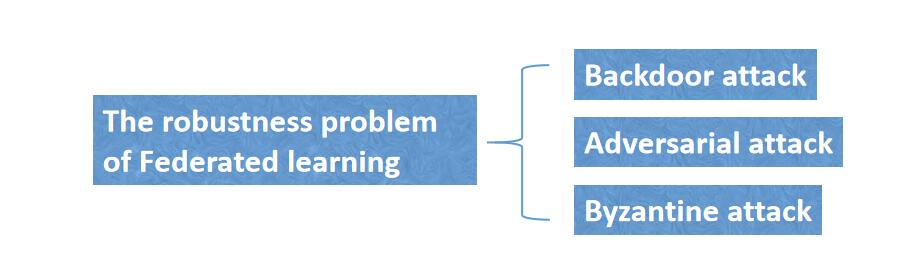
\includegraphics[width=0.8\linewidth,height=0.4\linewidth]{picture/f4.jpg}}
    \caption{The robust threat to federal learning}
    \label{fig2}
\end{figure}
And adversarial attacks can occur in federated learning when a malicious participant intentionally sends adversarial examples to the central server in an attempt to bias the model
towards their own interests. This can be particularly problematic in applications such as personalized advertising or credit scoring, where the malicious participant may be motivated
to gain an unfair advantage. Finally, Byzantine attacks involve one or more malicious participants in the federated learning process sending incorrect or misleading updates to the
central server to disrupt the training process\cite{b35}.

While federated learning can be vulnerable to certain types of attacks, there are techniques and approaches that can be used to improve the robustness and security of the process.
It is important to carefully consider these issues when designing and implementing federated learning systems\cite{b38},\cite{b39}.
For instance, knowledge distillation is a technique that can mitigate backdoor attacks by training a smaller\cite{b36},
distilled model using the output of the original model as the target labels.
This can help remove any backdoor triggers that may have been added to the original model, as the smaller model won't be able to identify them.
Another technique to mitigate backdoor attacks is model erasure\cite{b44}, where the model is trained to ignore specific input patterns that may be associated with the backdoor.
\begin{figure}[htbp]
    \centerline{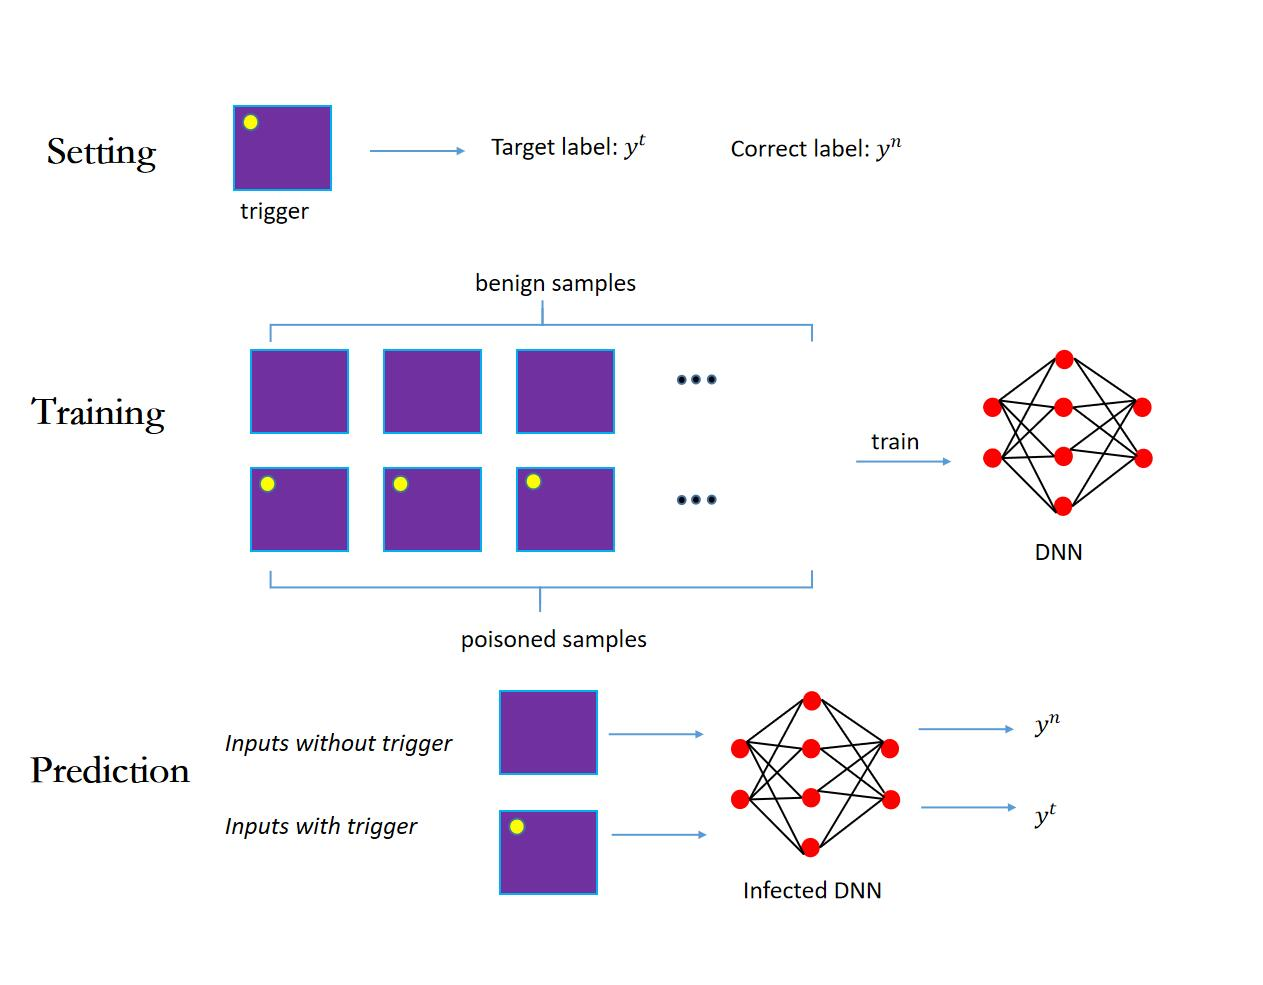
\includegraphics[width=0.8\linewidth,height=0.4\linewidth]{picture/f3.jpg}}
    \caption{Backdoor Attack}
    \label{fig3}
\end{figure}

Adversarial training is a technique that involves explicitly training the model to resist adversarial examples
by adding adversarial perturbations to the training data\cite{b31},\cite{b32}.
This can improve the model's ability to detect and resist adversarial attacks in federated learning settings.
\begin{figure}[htbp]
    \centerline{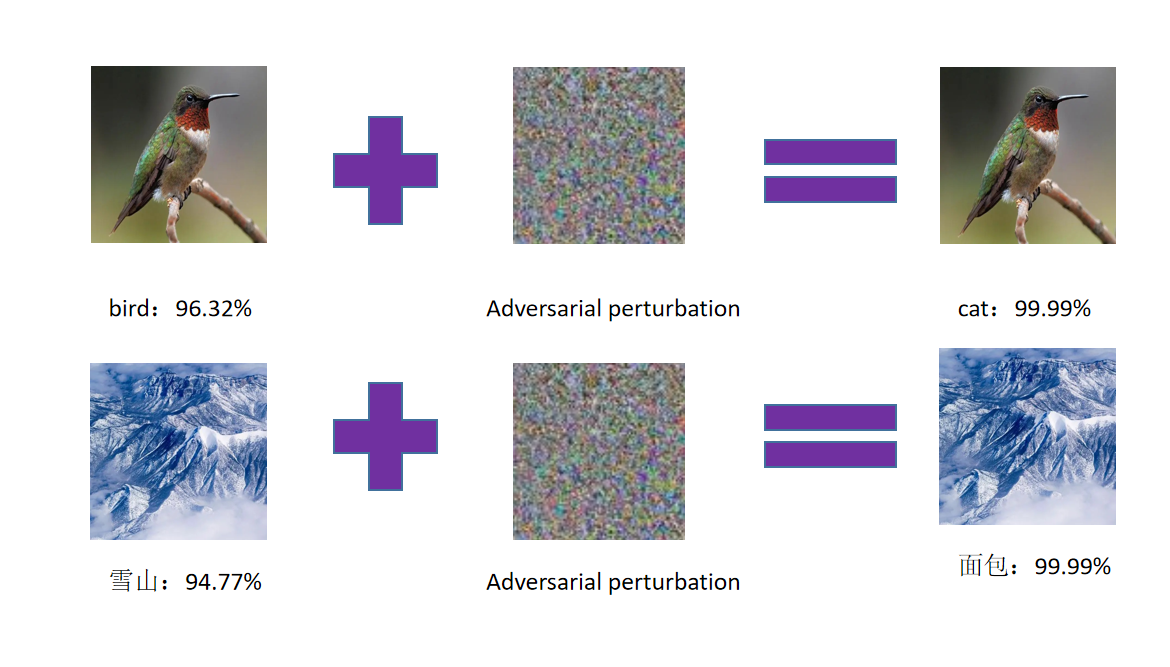
\includegraphics[width=0.8\linewidth,height=0.4\linewidth]{picture/f2.png}}
    \caption{Adversarial Attack}
    \label{fig4}
\end{figure}
Clustering can be used to identify malicious clients in federated learning systems subject to Byzantine attacks\cite{b35},\cite{b36}.
The idea is to group participating clients based on the similarity of their updates, and to identify any clients whose updates are significantly different from the others.
These clients can then be excluded from the training process, or their updates can be treated with greater suspicion to minimize the impact of their malicious behavior\cite{b37}.
\begin{figure}[htbp]
    \centerline{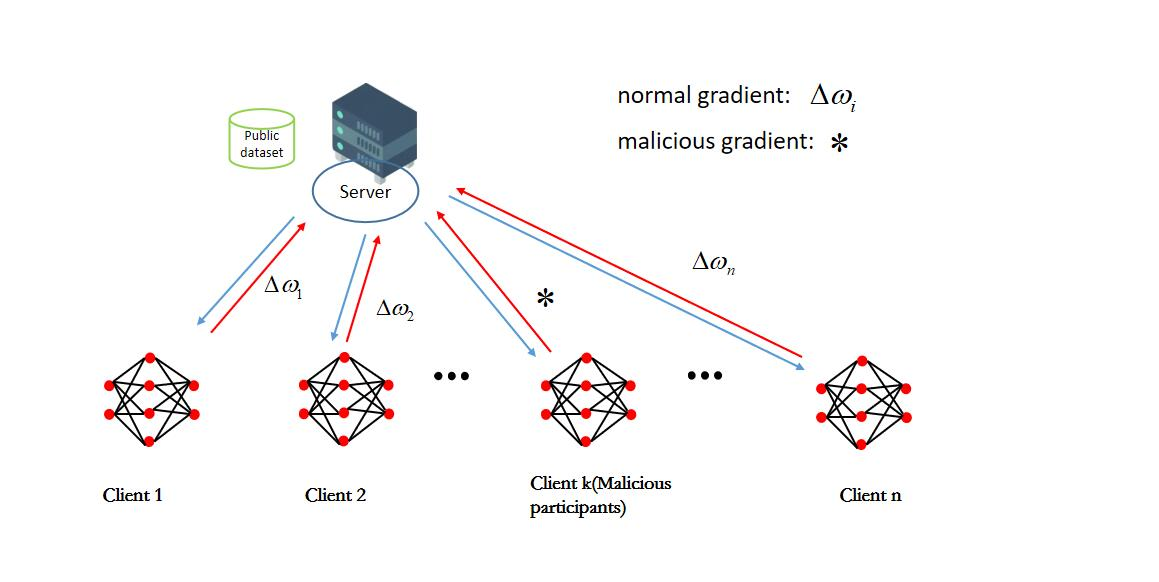
\includegraphics[width=0.8\linewidth,height=0.4\linewidth]{picture/f5.jpg}}
    \caption{Byzantine Attack}
    \label{fig5}
\end{figure}
This paper provides an overview of methods to increase the robustness of federated learning models, with the aim of enhancing the credibility and security of federated learning.
While previous work has addressed the security of federated learning\cite{b39},\cite{b40},\cite{b41},\cite{b42},\cite{b43}, it has primarily focused on privacy leakage or backdoor attacks,
with relatively few studies and reports on adversarial attacks. Building on prior work, this paper summarizes the attacks and defense methods of adversarial, backdoor,
and Byzantine attacks in federated learning. A new classification method is proposed, supplementing the deficiencies of previous work on adversarial attacks.
Moreover, this paper investigates a multi-level defense system against these attacks, and identifies open problems and future research directions for improving
the robustness of federated learning.

\section{Thraet Model}
Prior to delving into the details of the threats to federal learning, it is essential
to establish the connections between these threats based on different criteria.
Specifically, we can categorize these threats into two main stages:
the training phase and the inference phase. Additionally, we can
differentiate between untargeted attacks and targeted attacks based
on whether a specific target is present or not.\cite{b38},\cite{b39},\cite{b40},\cite{b41}.

\subsection{Training Phase and Inference Phase}
\subsubsection{Training Phase}Attacks that occur during the model training process are
intended to either disrupt or impact the federated learning model itself. Backdoors are
inserted into the model during the training phase to influence the resulting model outcomes\cite{b45},\cite{b46}.
On the other hand, Byzantine attacks disrupt the convergence of the model by utilizing malicious
clients or servers\cite{b29}.
\subsubsection{Inference Phase}Attacks that occur during the reasoning phase are
typically intended to alter the model's reasoning outcomes and deceive it
into generating incorrect outputs\cite{b47}. During the training stage, backdoor
attacks involve the insertion of a backdoor into the model, whereas
input deception models with triggers are utilized during the
reasoning stage to cause the model to generate incorrect results.
Adversarial attacks, on the other hand, leverage the model's vulnerability
to disturbances and utilize samples with adversarial perturbations as input
to the model, causing it to produce erroneous outcomes.

\subsection{Untargeted and Targeted}
\subsubsection{Untargeted attack}Untargeted attacks are designed to compromise
the integrity of the target model in an arbitrary manner.
Byzantine attack is one form of an untargeted attack that involves
uploading malicious gradients to the server in an arbitrary manner,
with the goal of causing the global model to fail\cite{b48},\cite{b49},\cite{b50},\cite{b51}.
\subsubsection{Targeted Attack}A targeted attack is executed with
the aim of inducing the model to produce the target label specified by the
adversary for specific testing examples, while keeping the testing error for
other testing examples unaffected\cite{b51}.

\section{Backdoor Attack}
A backdoor attack on deep neural networks entails surreptitiously implanting
a malicious backdoor within the model. This enables the model to function
normally when processing benign inputs, but triggers a pre-defined
malicious behavior when presented with a specific malicious trigger.
The first neural backdoor in centralized settings can be traced
back to 2013\cite{b52},\cite{b53}.

Due to the unique nature of federated learning, whereby the model is trained
on individual clients, it is more susceptible to backdoor attacks compared
to the general centralized training model. These types of attacks in federated
learning can be divided into two categories based on the different stages at
which the adversary inserts the backdoor into the training pipeline: data
poisoning attacks and model poisoning attacks.

\subsection{Data Poisoning Attack}
In data poisoning attacks, it is assumed that the adversary has full control
over the training data collection process of compromised clients. Then the poisoned
dataset typically consists of a combination of clean data with ground-truth labels
and data with backdoor triggers that have targeted labels.

\subsubsection{Invisible Poisoning}
In this context, the term "invisible" denotes the user's ability to execute
a backdoor attack on a sample without requiring any additional actions to
be performed on the sample itself.

Label flipping is a widely recognized attack in centralized machine learning (ML),
as demonstrated in previous research studies\cite{b54},\cite{b55}. In addition,
it is also a suitable method for the federated learning (FL) scenario,
given its adversarial goal and capabilities\cite{b56}.As shown in the picture,
some of the samples labeled "dog" are flipped to "bird" and the samples of "cat"
are flipped to "bread".

\begin{figure}[htbp]
    \centerline{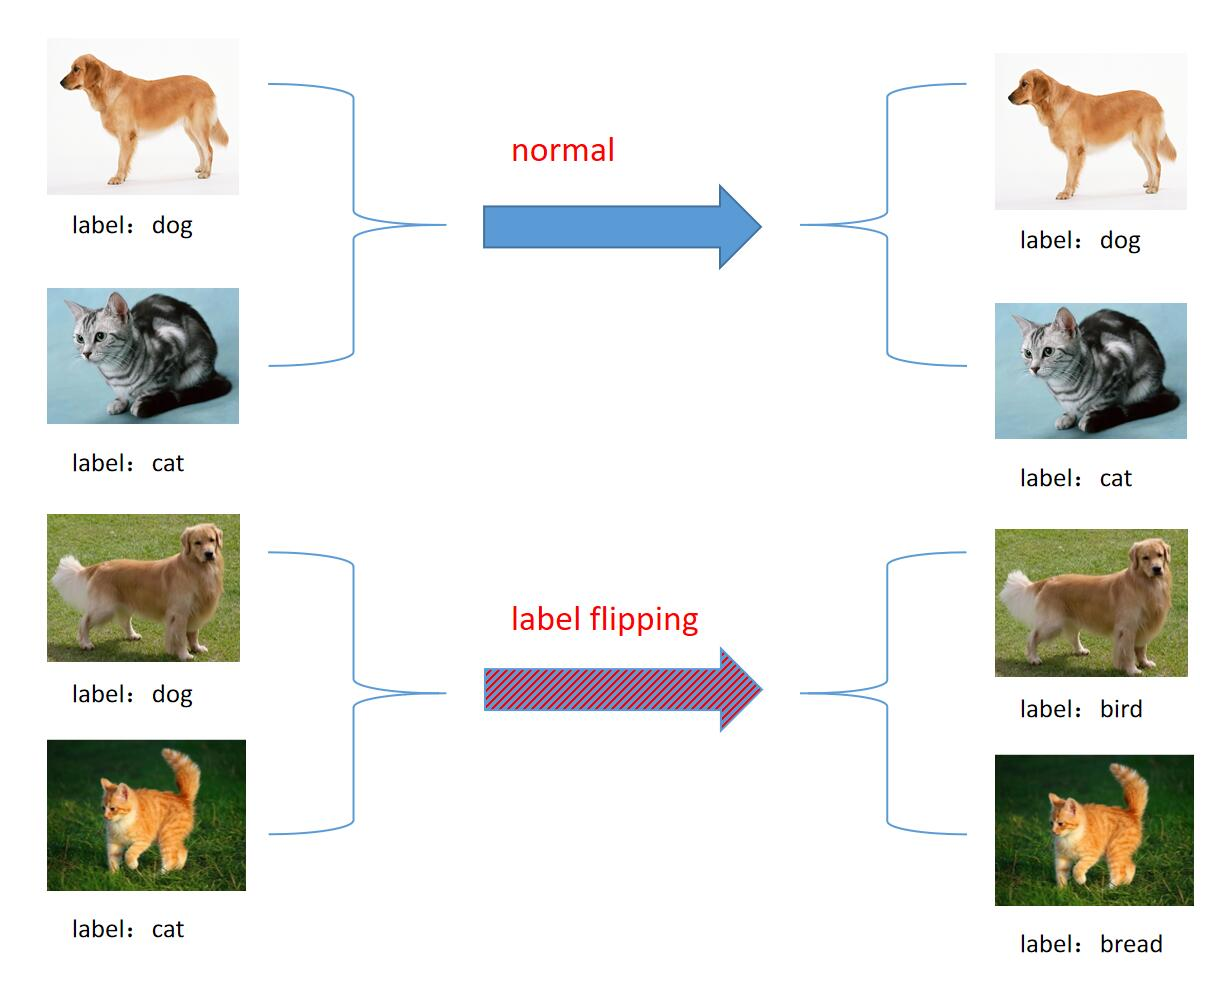
\includegraphics[width=0.8\linewidth,height=0.4\linewidth]{picture/f6.jpg}}
    \caption{Label Flipping}
    \label{fig6}
\end{figure}

Nevertheless, the label flipping technique has its limitations since it necessitates
modifying the label of the sample, making it less practical. Thus, an attack
technique that is more covert and can deceive manual inspection would be more
appealing in this scenario.A clean-label attack preserves the label of the poisoned data,
and the manipulated image still appears to be a benign sample\cite{b57},\cite{b58}. This type of attack
leverages feature collision, where the crafted poison examples continue to
resemble the source instance in visual appearance, while being closer to the
targeted instance in the latent feature space.

\begin{figure}[htbp]
    \centerline{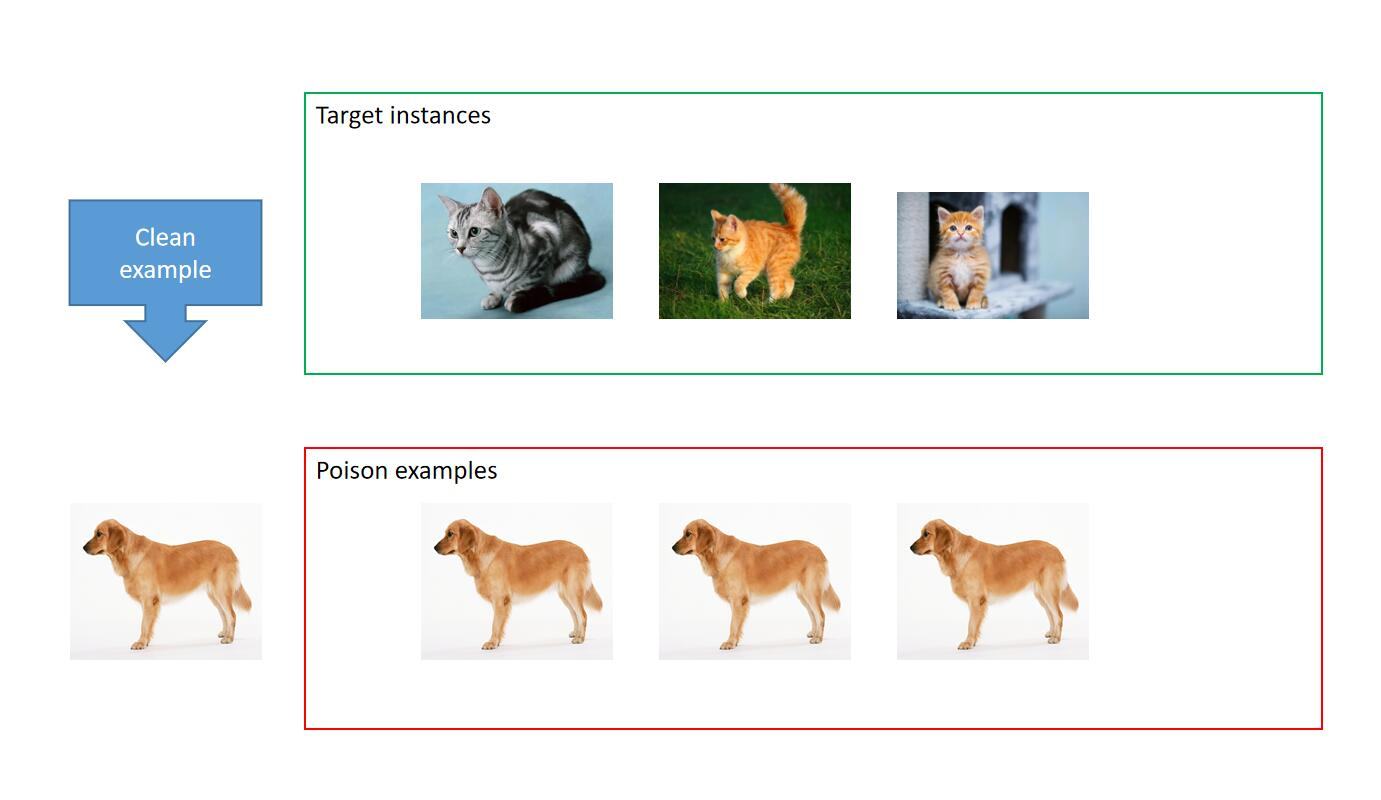
\includegraphics[width=0.8\linewidth,height=0.4\linewidth]{picture/f7.jpg}}
    \caption{Clean Label Attack}
    \label{fig7}
\end{figure}

\subsubsection{Visible Poisoning}
Early methods of  backdoor attacks in federated learning can rely on a single trigger,
meaning that all corrupted clients inject the same trigger into their local
training dataset. The triggers employed in this method are usually predetermined,
such as a square located at redundant pixels in the image. During reasoning,
the inserted trigger is used on a malicious client to activate the aggregation model\cite{b24},\cite{b27}.
While the effectiveness of inserting the backdoor has been shown to be significant,
the aforementioned approach merely transfers backdoor attacks from centralized
learning directly to federated learning, without fully leveraging
the distributed nature of the latter. This is
because the same trigger is embedded in all adversarial clients.

Xie et al. \cite{b59} proposed a distributed backdoor attack (DBA) that decomposes a global t
rigger pattern, similar to a centralized attack, into local patterns and embeds
them into different malicious clients. Compared to traditional methods that insert
the same trigger, DBA is more efficient and covert due to its hidden local
trigger mode, making it easier to bypass robust aggregation rules.

\begin{figure}[htbp]
    \centerline{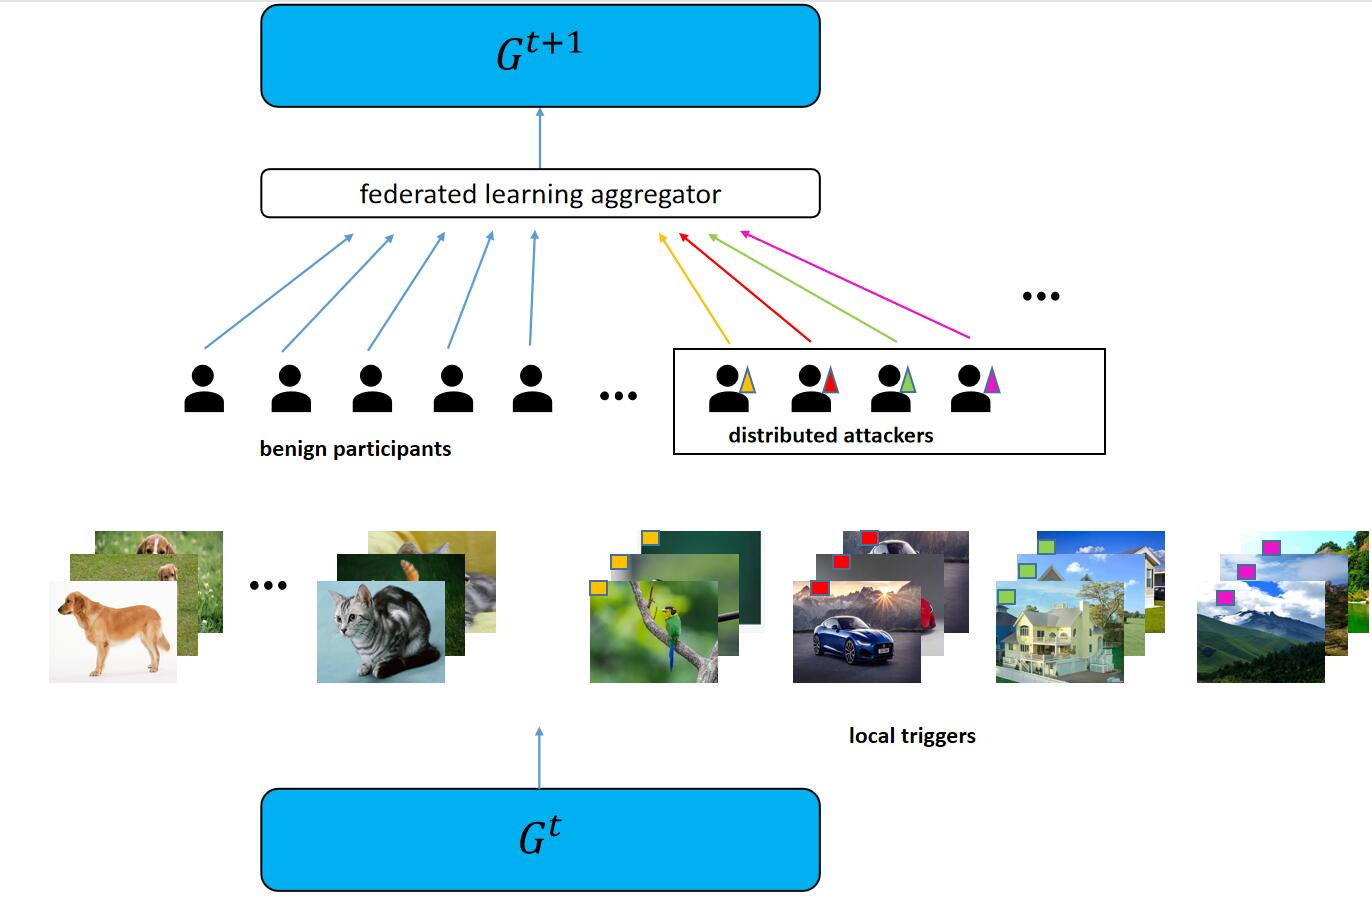
\includegraphics[width=0.8\linewidth,height=0.4\linewidth]{picture/f8.jpg}}
    \caption{Distributed Backdoor Attack}
    \label{fig8}
\end{figure}

In order to enhance the effectiveness of data poisoning attacks,
dynamic triggers have been proposed and applied. Salem et al \cite{b60} conducted a
clear and systematic study on the feasibility of dynamic flip-flops,
which can facilitate the backdoor attacks by generating antagonistic
network algorithms to create triggers. This way, the same tags can be
hijacked with different trigger patterns that share similar potential
representations and positions. Et al \cite{b61} also conducted a direct
investigation of dynamic triggers. These triggers can be flexibly produced
during the physical attack phase, as they maintain their effectiveness even
under substantial changes. The results of the study show that dynamically
triggered backdoor attacks are more powerful, and they require new techniques
to be defeated because they break the static trigger hypothesis of most current
defense systems.

Despite the potential threat of data poisoning attacks in federated learning,
they face many practical limitations due to the unique distributed characteristics of this approach\cite{b25}.
This is because the data distribution and model aggregation steps in federated learning tend to neutralize
most of the contributions of the backdoor model, leading to rapid forgetting of the backdoor by the global model.
In light of this situation, Wang et al.\cite{b25} proposed selecting poisoning samples from edge data to reduce the
forgetting effect caused by model updating. Dai et al.\cite{b64} proposed a new backdoor attack called Champeleon,
which enables attackers to create more persistent visual backdoors by adapting
to peer-to-peer images. The durability of the backdoor largely depends
on the existence of two types of identical benign images that are closely
related to the toxic image: 1) interferers, which are images that share
the same original tag as the toxic image, and 2) facilitators, which are
images with the target back tag. Interferers can cause update conflicts
between toxic updates and benign updates, which may reduce the accuracy of
the backdoor. Conversely, facilitators can help reintroduce backdoor
information into the federated learning model and mitigate the catastrophic
forgetting effect after the attacker leaves the training process. Inspired by
these observations, Champeleon is designed to amplify these effects and enhance
the durability of the backdoor.

\subsection{Model Poisoning Attack}
To address the limitations of data poisoning attacks, we can not only focus on
improving the data poisoning technology itself, but also explore the potential
of model poisoning techniques. Since the average method is the most widely-used
approach for aggregating local updates from clients, a simple way to amplify
the backdoor effect is to prioritize updates from adversarial clients over
those from benign clients.

Bagdasaryan et al.\cite{b24} proposed the first backdoor attack against federated learning.
Their approach involves training a backdoor model that closely resembles the global
model, which is then used to replace the latest global model.
To improve the effectiveness of this replacement, they slow down
the learning rate to extend the lifespan of the backdoor model, and add an
anomaly detection term to the loss function to avoid detection. This
strategy requires careful evaluation of the global parameters and performs
better when the global model is close to convergence.

Zhou et al.\cite{b63} proposed an optimization-based model poisoning attack that
involves injecting adversarial neurons into the redundant space of a neural network
to maintain the attack's concealment and persistence. To identify the redundant
space, the Hessian matrix is used to measure the update distance and direction of each neuron's main task (i.e. "importance").
An additional term is then added to the loss function to prevent poisoned neurons from being injected
in locations that are particularly relevant to the main task.
In a similar vein, Zhang et al.\cite{b62}
proposed a persistent backdoor attack called Neurotoxin. This method
relies on the empirical observation that the norm of a stochastic gradient
is primarily concentrated in a small number of "heavy hitter" coordinates.
Neurotoxin identifies these heavy hitters using the top-k heuristic and
avoids them. By avoiding directions that are most likely to receive large
updates from benign devices, the chance of the backdoor being erased is mitigated.

Sun et al. \cite{b65}proposed a distance-aware attack (ADA), which enhances poisoning attacks
by identifying optimized target classes in the feature space. They addressed the challenge of
limited prior knowledge of customer data that competitors may face. To overcome this problem,
ADA infers the pairwise distances between different categories in the potential feature space
from the shared model parameters using backward error analysis. They conducted an extensive
empirical evaluation of ADA by varying attack frequency in three different image classification
tasks. As a result, ADA successfully improved the attack performance by 1.8 times in the most
challenging cases with attack frequency of 0.01x.

\subsection{Summary Of Federated Backdoor Attack}
The primary challenge of backdoor attacks in federated learning is how
to leverage the distributed nature of this approach, evade detector checks,
and ensure the persistence of the backdoors during multiple rounds of update
iterations. We identify three research directions for federated backdoor
attacks: using multiple malicious clients to insert backdoor attacks,
combining generation technology with backdoor attacks, and conducting
research on persistent backdoor attacks in federated learning.

\section{Defenses against Backdoor Attack}
To mitigate the problem of backdoor attacks in
federated learning, various defensive techniques have been proposed.
Given that we previously categorized backdoor attacks as data poisoning
attacks and model poisoning attacks, we will now discuss defensive strategies
for each of these attack types.

\subsection{Defense Against Data Poisoning}
The simplest approach is to filter out poisoned data samples,
which aims to remove the poisoned samples from the training dataset.
After the filtering process, only benign samples or purified poisoned
samples are used during the training process, thus eliminating the
creation of a backdoor from the source.

Tran et al.\cite{b67} were the first to investigate methods for filtering out malicious
samples from the training set. They demonstrated that poisoned samples tend to
leave detectable traces within the covariance range of the feature representation.
Exploiting this insight, it is possible to filter out poisoned samples from
the training set.Zeng et al. \cite{b68} revealed that poisoned samples of
existing attacks had some high-frequency artifacts even if their trigger
patterns are invisible in the input space. Based on this observation,
they designed a simple yet effective filtering method based on those artifacts.
Similarly, Chen et al. \cite{b69}proposed a two-stage filtering approach.
In the first stage, activation values of samples in each class are clustered
into two groups, and in the second stage, it is determined which clusters
correspond to poisoned samples.

As is well known, backdoors are triggered during the inference stage.
Filtering out malicious samples from the testing samples during the inference stage can prevent the backdoor
from being activated. Gao et al. \cite{b71} proposed to filter attacked samples by overlaying various image patterns
on suspicious samples. The smaller the randomness of the input perturbation prediction, the higher the probability
that the suspicious sample is attacked. In \cite{b72}, Subedar et al. used model uncertainty to distinguish between
benign and attacked samples. Later, Du et al. \cite{b73} regarded filtering as outlier detection and proposed a
differential privacy-based filtering method. Recently, \cite{b74} proposed a lightweight method that can filter
attacked samples or prior hypotheses of trigger patterns without labeled samples.
However, Tang et al.\cite{b70} demonstrated that
simple target contamination can result in malicious and benign samples being
indistinguishable in the feature representation space. Therefore, most
sample filtering techniques are ineffective.

Based on data-driven defense methods, in addition to filtering out samples,
it is also possible to consider directly preprocessing the samples,
specifically by erasing any backdoors within them to prevent them from being embedded in the model.
Liu et al.\cite{b75} proposed a pre-trained autoencoder as a preprocessor to prevent malicious samples from embedding backdoors
by preprocessing the input samples without affecting data classification accuracy.

\begin{figure}[htbp]
    \centerline{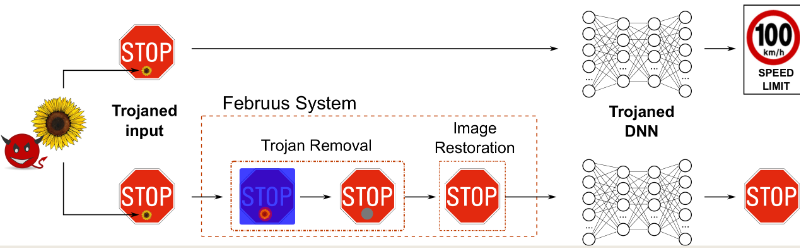
\includegraphics[width=0.8\linewidth,height=0.4\linewidth]{picture/f9.png}}
    \caption{Overview of the Februus System.}
    \label{fig9}
\end{figure}
Doan et al. \cite{b76}proposed a two-stage image processing method called Februus, in which,
in the first stage, Februus uses GradCAM to identify influential regions, which are then
removed and replaced with a neutral color frame. Subsequently, Februus uses a GAN-based
repair method to reconstruct the masked regions to mitigate their adverse effects (such as benign accuracy reduction).
Li et al. \cite{b77} discussed the properties of existing poisoning-based static trigger mode attacks. They demonstrated
that the attack performance may sharply decrease if the appearance or location of the trigger is slightly changed.
Based on this observation, they recommended using spatial transformations (such as contraction, flipping)
for defense. Compared to previous methods, this method is more efficient because it requires almost no additional computational cost.

\subsection{Defense Against Model Poisoning}  
\subsubsection{Filtering}
Similar to defense methods against poisoned data, defense methods against poisoned models also begin with model filtering. 
Fung et al. proposed FoolsGold \cite{b78}, which checks for and eliminates suspicious updates during local updates. 
FoolsGold is based on the fact that when a global model is trained by a group of attackers, they will submit updates with 
the same backdoor objectives throughout the training process, resulting in similar behavior.   

However, this similarity does not occur among honest participants because each user's training dataset is unique and not shared with others. 
Therefore, malicious attackers can be separated from benign attackers through gradient updates. After detecting such anomalies, 
FoolGold maintains the learning rate of benign users (submitting only unique gradient updates) and reduces the learning rate of malicious users 
(repeatedly uploading similar gradient updates) to mitigate backdoor attacks. However, experimental results show that 
FoolsGold cannot defend against adaptive attacks. Li et al. \cite{b79} proposed a spectral anomaly detection framework for a 
central aggregator that detects and erases backdoor model updates through strong detection model detection. 
The key idea of spectral anomaly detection is that there is a significant difference between the embedding 
of benign updates and backdoor updates in a low-dimensional latent space. One practical method for approximating 
low-dimensional embedding is to build a model using an encoder-decoder structure, where the encoder takes 
in the raw update and returns a low-dimensional embedding, and the decoder is fed the embedding and outputs 
the generation error. After training the encoder-decoder model on benign updates, it can be used to identify 
backdoor updates, generating errors much higher than benign errors; malicious updates will be excluded from 
the aggregation process. However, this defense method cannot handle multi-trigger backdoor attacks, i.e., 
injecting various backdoors simultaneously.   

Nguyen et al. proposed FlGuard \cite{b80}, a two-layer defense method that checks 
for locally updated updates with clear backdoor effects and eliminates residual backdoors through pruning, smoothing, and noise 
addition. Unlike FoolsGold\cite{b78}, it also applies to multi-trigger backdoor attacks while maintaining high prediction accuracy for benign primary tasks. 
Additionally, FLDetector \cite{b81} proposed a method to detect malicious clients by checking the consistency of model updates. Essentially, 
the server predicts the client's model update based on past updates in each iteration. If the model update received by the client 
differs significantly from the predicted update over multiple iterations, the client is marked as malicious. Overall, the focus of 
these methods is mainly divided into two types: the first is to remove toxic updates from malicious clients before model aggregation, 
and the second is to reduce the impact of malicious clients on the aggregated model, such as reducing the learning rate of suspicious clients.

\subsubsection{Robust Training}  
After filtering techniques, another class of techniques aims to directly mitigate backdoor attacks during model training through robust joint training. 
Differential privacy algorithms have been shown to be effective against backdoors \cite{b82}, but they may compromise model performance under data imbalance 
commonly found in federated learning \cite{b83}. DP-FedAvg \cite{b84} (Central-DP) is a differential private aggregation strategy that eliminates 
outliers by clipping the norm of model updates and adding Gaussian noise, but the required amount of noise significantly reduces 
task accuracy. Sun et al. \cite{b27} proposed weak DP, which adds sufficient Gaussian noise to defeat backdoors while maintaining task accuracy, 
but it is ineffective against constraint-based backdoor attacks \cite{b25}. 
Additionally, DP-based defenses can potentially impact the benign performance of the global model, 
as the clipping factor also changes the weights of benign model updates.   

In addition to DP-based defenses, Andreina et al. \cite{b85}proposed Feedback-based Federated Learning (BaFFle) to eliminate backdoors.  
The key idea of BaFFle is to leverage participants to verify the global model. BaFFle includes a super-digit verification process for each 
round of federated learning. Specifically, each selected participant checks the current global model by computing a verification function on 
their secret data and reports to the central server whether the model is backdoored or not. The central server then decides whether 
to accept or reject the current global model based on feedback from all users. The verification function compares the error rate of 
a specific class of the current global model with the error rate of previously accepted global models. If the error rate is significantly different, 
the central server rejects the current global model as it may be backdoored and issues an alert. Unlike anomaly detection, BaFFle is compliant with secure aggregation.

Considering that all of the above defense works lack robustness certification, 
Xie et al. \cite{b86} proposed the first general defense framework CRFL for training certifiably robust FL models against backdoor attacks. 
CRFL controls the model smoothness through pruning and smoothing of model parameters and generates sample robustness 
certification against amplitude-limited backdoor attacks. Smoothness and perturbation methods are also used as an 
additional component to constrain the L2 norm of individual updates to enhance defense performance \cite{b87}. 
In addition, the FL-WBC \cite{b88} method aims to identify the fragile parameter space in FL and perturb it 
during client training. FL-WBC also provides robustness guarantees against backdoor attacks and convergence guarantees for FedAvg. 
These developments demonstrate promising steps towards improving FL's robustness against backdoor attacks. In FLARE \cite{b89}, a trust 
evaluation method is proposed that calculates a trust score for each model update based on the difference between all model updates and 
their penultimate layer representation values. FLARE assumes that most clients are trustworthy and assigns low scores 
to updates that are far from benign update clusters. The model updates are then aggregated with their trust scores as 
weights and the global model is updated accordingly.

In \cite{b98}, the concept of anti-backdoor learning is introduced, which involves training a clean model given infected data, 
dividing the overall learning task into a dual task of learning the clean part of the data and the backdoor part. 
The article leverages two inherent weaknesses of backdoor attacks: models learn backdoor data faster than clean data, 
and the stronger the attack, the faster the model converges on the backdoor data. Additionally, backdoor tasks are mutually 
associated with specific classes. Based on these two weaknesses, a generic learning scheme is proposed to automatically prevent 
backdoor attacks during training. A two-stage gradient ascent mechanism is introduced to isolate and separate backdoor samples 
from the target class during the early training stage and break the association between backdoor samples and the target class during the later training stage.
\subsubsection{Model Reconstruction}  
The model reconstruction-based approach aims to eliminate hidden backdoors in infected models by directly modifying suspicious models. 
Therefore, even if triggers are included in the attack samples, the reconstructed model will still correctly predict them because 
the hidden backdoors have been removed.

As mentioned earlier, the forgetting mechanism of federated backdoor attacks means that as training and model aggregation progress, 
the backdoor will be forgotten in successive iterations. As a defense, this forgetting mechanism can also be utilized to create many defensive methods.

Zeng et al. \cite{b90}defined multiple training as a min-max problem and used implicit hyper-gradients to 
explain the interdependence between internal and external optimization.  
In \cite{b91}, Zhao et al. showed that hidden backdoors infecting DNNs can be repaired using pattern connectivity techniques with a certain number of benign samples. 
Yoshida et al.  and Li et al. \cite{b92} perturbed backdoor-related neurons based on the distillation process, reconstructed (infected) DNNs using knowledge 
distillation techniques , and thus removed hidden backdoors.
In addition to directly eliminating hidden backdoors, defense based on trigger synthesis first 
synthesizes backdoor triggers, and then in the second phase, eliminates hidden backdoors by suppressing the influence of triggers. 
These defenses have some similarities in the second phase with reconstruction-based defenses. For example, 
pruning and retraining are commonly used techniques to remove hidden backdoors in both defenses. However, 
compared to reconstruction-based defenses, the trigger-based defenses' trigger information makes the removal process more effective and efficient.

A GAN-based method was proposed in \cite{b93} to synthesize trigger distributions. 
In \cite{b94}, they showed that the detection process used in \cite{b95} to determine synthesized 
triggers has several failure modes and proposed a new defense method based on this observation. 
Additionally, Cheng et al. \cite{b96} revealed that the '∞ norm of activation values can be used to 
distinguish backdoor-related neurons based on synthesized triggers. Therefore, they propose performing an 
'∞-based neuron pruning to remove neurons with high activation values in response to triggers. 
Similarly, Aiken et al.\cite{b97} also propose removing hidden backdoors 
by pruning DNNs based on synthesized triggers from another perspective. 


\section{Byzantine Attack}
\section{Defenses against Byzantine Attack}
\section{Adversarial Attack}
Both adversarial attacks and backdoor attacks are techniques used to modify benign
testing samples in order to make models misbehave during the inference process.
While adversarial perturbations are sample-agnostic in universal adversarial attacks,
these attacks can seem similar to backdoor attacks. Consequently, researchers who are
not familiar with backdoor attacks may question their significance, as these attacks
require additional controls on the training process to some extent.
However, despite certain similarities, these attacks have essential differences.
Firstly, adversarial attackers need to control the inference process (to a certain extent)
but not the training process of models. They need to query the model results or even gradients
multiple times to generate adversarial perturbations by optimization given a fixed targeted model.
On the other hand, backdoor attackers require modifying some training stages (e.g., data collection,
model training) without any additional requirements in the inference process.
Secondly, from the perspective of attacked samples, backdoor attackers use known
(i.e., non-optimized) perturbations, whereas adversarial attackers need to obtain them through
the optimization process based on the output of the model. This optimization in adversarial attacks
requires multiple queries, making them unable to be real-time in many cases.
Finally, the mechanisms of these attacks are also essentially different.
Adversarial vulnerability results from the differences in behaviors of models and humans,
while backdoor attackers utilize the excessive learning ability of deep neural networks (DNNs)
to build a latent connection between trigger patterns and target labels. Recently,
there have been some works studying the latent connection between adversarial attacks
and backdoor attacks. For example, Weng et al. \cite{b66}empirically demonstrated that defending
against adversarial attacks via adversarial training may increase the risks of backdoor attacks.



\section{Defenses against Adversarial Attack}
\section{Hrbrid Defenses}
\section{Advanced Research and Problems}
\section{Conclusion}




\begin{thebibliography}{00}
    \bibitem{b1} M. Goddard, The EU General Data Protection Regulation (GDPR): European regulation that has a global impact, International Journal of Market Research 59 (2017) 703~705.
    \bibitem{b2} O. Gómez-Carmona, D. Casado-Mansilla, F. A. Kraemer, D. L. de Ipiña, J. GarcíaZubia, Exploring the computational cost of machine learning at the edge for human-centric internet of things, Future Generation Computer Systems 112 (2020) 670–683.
    \bibitem{b3} J. Zhang, D. Tao, Empowering things with intelligence: A survey of the progress, challenges, and opportunities in artificial intelligence of things, IEEE Internet of Things Journal 8 (2021) 7789–7817.
    \bibitem{b4} C. Ma, J. Koneˇcný, M. Jaggi, V. Smith, M. Jordan, P. Richtárik, M. Takáˇc, Distributed optimization with arbitrary local solvers, Optimization Methods and Software 32 (2017) 813–848.
    \bibitem{b5} Brendan McMahan, Eider Moore, Daniel Ramage, Seth Hampson, and Blaise Aguera y Arcas. Communication-Efficient Learning of Deep Networks from Decentralized Data. In Proceedings of the 20th International Conference on Artificial Intelligence and Statistics, volume 54 of Proceedings of Machine Learning Research, pages 1273–1282. PMLR, 20–22 Apr 2017.
    \bibitem{b6} GlobalFederatedLearningMarketbyApplication (Drug Discovery, Industrial IoT, Risk Management), Vertical (Healthcare  Life Sciences, BFSI, Manufacturing, Automotive Transportation, Energy  Utilities), and Region - Forecast to 2028, "researchandmarkets.com", Accessed date: May 12, 2023.
    \bibitem{b7} Q. Yang, Y. Liu, Y. Cheng, Y. Kang, T. Chen, H. Yu, Federated Learning, Synthesis Lectures on Artificial Intelligence and Machine Learning, 2019.
    \bibitem{b8} M. Househ, E. Borycki, and A. Kushniruk. Multiple Perspectives on Artificial Intelligence in Healthcare. Springer, 2021.
    \bibitem{b9} R. Rau, R. Wardrop, and L. Zingales. The Palgrave Handbook of Technological Finance. Springer, 2021.
    \bibitem{b10} Fang, Xiuwen, and Mang Ye. "Robust federated learning with noisy and heterogeneous clients." Proceedings of the IEEE/CVF Conference on Computer Vision and Pattern Recognition. 2022.
    \bibitem{b11} Tang, Zhenheng, et al. "Virtual homogeneity learning: Defending against data heterogeneity in federated learning." International Conference on Machine Learning. PMLR, 2022.
    \bibitem{b12} Kairouz, Peter, et al. "Advances and open problems in federated learning." Foundations and Trends® in Machine Learning 14.1~2 (2021): 1-210.
    \bibitem{b13} Yang, Qiang, et al. "Federated machine learning: Concept and applications." ACM Transactions on Intelligent Systems and Technology (TIST) 10.2 (2019): 1-19.
    \bibitem{b14} Huang, Wei, et al. "Fairness and accuracy in horizontal federated learning." Information Sciences 589 (2022): 170-185.
    \bibitem{b15} Liu, Yang, et al. "Vertical federated learning." arXiv preprint arXiv:2211.12814 (2022).
    \bibitem{b16} Ghosh, Avishek, et al. "An efficient framework for clustered federated learning." Advances in Neural Information Processing Systems 33 (2020): 19586-19597.
    \bibitem{b17} Briggs, Christopher, Zhong Fan, and Peter Andras. "Federated learning with hierarchical clustering of local updates to improve training on non-IID data." 2020 International Joint Conference on Neural Networks (IJCNN). IEEE, 2020.
    \bibitem{b18} Hsu, Tzu-Ming Harry, Hang Qi, and Matthew Brown. "Federated visual classification with real-world data distribution." Computer Vision ECCV 2020: 16th European Conference, Glasgow, UK, August 23–28, 2020, Proceedings, Part X 16. Springer International Publishing, 2020.
    \bibitem{b19} Wahab, Omar Abdel, et al. "Federated machine learning: Survey, multi-level classification, desirable criteria and future directions in communication and networking systems." IEEE Communications Surveys and Tutorials 23.2 (2021): 1342-1397.
    \bibitem{b20} Yang, Shengwen, et al. "Parallel distributed logistic regression for vertical federated learning without third-party coordinator." arXiv preprint arXiv:1911.09824 (2019).
    \bibitem{b21} Deng, Yuyang, Mohammad Mahdi Kamani, and Mehrdad Mahdavi. "Distributionally robust federated averaging." Advances in neural information processing systems 33 (2020): 15111-15122.
    \bibitem{b22} Sun, Tao, Dongsheng Li, and Bao Wang. "Decentralized federated averaging." IEEE Transactions on Pattern Analysis and Machine Intelligence 45.4 (2022): 4289-4301.
    \bibitem{b23} Fallah, Alireza, Aryan Mokhtari, and Asuman Ozdaglar. "Personalized federated learning: A meta-learning approach." arXiv preprint arXiv:2002.07948 (2020).
    \bibitem{b24} Bagdasaryan, Eugene, et al. "How to backdoor federated learning." International conference on artificial intelligence and statistics. PMLR, 2020.
    \bibitem{b25} Wang, Hongyi, et al. "Attack of the tails: Yes, you really can backdoor federated learning." Advances in Neural Information Processing Systems 33 (2020): 16070-16084.
    \bibitem{b26} Gong, Xueluan, et al. "Backdoor attacks and defenses in federated learning: State-of-the-art, taxonomy, and future directions." IEEE Wireless Communications (2022).
    \bibitem{b27} Sun, Ziteng, et al. "Can you really backdoor federated learning?." arXiv preprint arXiv:1911.07963 (2019).
    \bibitem{b28} Ozdayi, Mustafa Safa, Murat Kantarcioglu, and Yulia R. Gel. "Defending against backdoors in federated learning with robust learning rate." Proceedings of the AAAI Conference on Artificial Intelligence. Vol. 35. No. 10. 2021.
    \bibitem{b29} Fang, Minghong, et al. "Local model poisoning attacks to {Byzantine-Robust} federated learning." 29th USENIX security symposium (USENIX Security 20). 2020.
    \bibitem{b30} Guo, Shangwei, et al. Byzantine-Resilient Decentralized Stochastic Gradient Descent.
    \bibitem{b31} Zizzo, Giulio, et al. "Fat: Federated adversarial training." arXiv preprint arXiv:2012.01791 (2020).
    \bibitem{b32} Chen, Chen, et al. "Calfat: Calibrated federated adversarial training with label skewness." Advances in Neural Information Processing Systems 35 (2022): 3569-3581.
    \bibitem{b33} Li, Xiaoxiao, Zhao Song, and Jiaming Yang. "Federated adversarial learning: A framework with convergence analysis." International Conference on Machine Learning. PMLR, 2023.
    \bibitem{b34} Zhang, Jie, et al. "Delving into the adversarial robustness of federated learning." arXiv preprint arXiv:2302.09479 (2023).
    \bibitem{b35} Prakash, Saurav, and Amir Salman Avestimehr. "Mitigating byzantine attacks in federated learning." arXiv preprint arXiv:2010.07541 (2020).
    \bibitem{b36} Huang, Hanxun, et al. "Distilling Cognitive Backdoor Patterns within an Image." arXiv preprint arXiv:2301.10908 (2023).
    \bibitem{b37} Blanchard, Peva, et al. "Machine learning with adversaries: Byzantine tolerant gradient descent." Advances in neural information processing systems 30 (2017).
    \bibitem{b38} Lyu, Lingjuan, et al. "Privacy and robustness in federated learning: Attacks and defenses." IEEE transactions on neural networks and learning systems (2022).
    \bibitem{b39} Guo, Shangwei, et al. "Robust and privacy-preserving collaborative learning: A comprehensive survey." arXiv preprint arXiv:2112.10183 (2021).
    \bibitem{b40} Enthoven, David, and Zaid Al-Ars. "An overview of federated deep learning privacy attacks and defensive strategies." Federated Learning Systems: Towards Next-Generation AI (2021): 173-196.
    \bibitem{b41} Rodríguez-Barroso, Nuria, et al. "Survey on federated learning threats: Concepts, taxonomy on attacks and defences, experimental study and challenges." Information Fusion 90 (2023): 148-173.
    \bibitem{b42} Tariq, Asadullah, et al. "Trustworthy Federated Learning: A Survey." arXiv preprint arXiv:2305.11537 (2023).
    \bibitem{b43} Zhang, Yifei, et al. "A Survey of Trustworthy Federated Learning with Perspectives on Security, Robustness, and Privacy." arXiv preprint arXiv:2302.10637 (2023).
    \bibitem{b44} Dal Fabbro, Nicolò, Aritra Mitra, and George J. Pappas. "Federated TD Learning over Finite-Rate Erasure Channels: Linear Speedup under Markovian Sampling." IEEE Control Systems Letters (2023).
    \bibitem{b45} Miao, Chenglin, et al. "Towards data poisoning attacks in crowd sensing systems." Proceedings of the Eighteenth ACM International Symposium on Mobile Ad Hoc Networking and Computing. 2018.
    \bibitem{b46} Zhang, Hengtong, et al. "Data poisoning attack against knowledge graph embedding." arXiv preprint arXiv:1904.12052 (2019).
    \bibitem{b47} Barreno, Marco, et al. "Can machine learning be secure?." Proceedings of the 2006 ACM Symposium on Information, computer and communications security. 2006.
    \bibitem{b48} Lamport, Leslie, Robert Shostak, and Marshall Pease. "The Byzantine generals problem." Concurrency: the works of leslie lamport. 2019. 203-226.
    \bibitem{b49} Xie, Cong, Oluwasanmi Koyejo, and Indranil Gupta. "Fall of empires: Breaking byzantine-tolerant sgd by inner product manipulation." Uncertainty in Artificial Intelligence. PMLR, 2020.
    \bibitem{b50} Bernstein, Jeremy, et al. "signSGD with majority vote is communication efficient and fault tolerant." arXiv preprint arXiv:1810.05291 (2018).
    \bibitem{b51} Damaskinos, Georgios, et al. "Aggregathor: Byzantine machine learning via robust gradient aggregation." Proceedings of Machine Learning and Systems 1 (2019): 81-106.
    \bibitem{b52} Geigel, Arturo. "Neural network trojan." Journal of Computer Security 21.2 (2013): 191-232.
    \bibitem{b53} Gu, Tianyu, Brendan Dolan-Gavitt, and Siddharth Garg. "Badnets: Identifying vulnerabilities in the machine learning model supply chain." arXiv preprint arXiv:1708.06733 (2017).
    \bibitem{b54} Shen, Shiqi, Shruti Tople, and Prateek Saxena. "Auror: Defending against poisoning attacks in collaborative deep learning systems." Proceedings of the 32nd Annual Conference on Computer Security Applications. 2016.
    \bibitem{b55} Steinhardt, Jacob, Pang Wei W. Koh, and Percy S. Liang. "Certified defenses for data poisoning attacks." Advances in neural information processing systems 30 (2017).
    \bibitem{b56} Tolpegin, Vale, et al. "Data poisoning attacks against federated learning systems." Computer Security ESORICS 2020: 25th European Symposium on Research in Computer Security, ESORICS 2020, Guildford, UK, September 14–18, 2020, Proceedings, Part I 25. Springer International Publishing, 2020.
    \bibitem{b57} Shafahi, Ali, et al. "Poison frogs! targeted clean-label poisoning attacks on neural networks." Advances in neural information processing systems 31 (2018).
    \bibitem{b58} Zhu, Chen, et al. "Transferable clean-label poisoning attacks on deep neural nets." International Conference on Machine Learning. PMLR, 2019.
    \bibitem{b59} Xie, Chulin, et al. “DBA: Distributed Backdoor Attacks against Federated Learning.” International Conference on Learning Representations,International Conference on Learning Representations, Apr. 2020.
    \bibitem{b60} Salem, Ahmed, et al. "Dynamic backdoor attacks against machine learning models." 2022 IEEE 7th European Symposium on Security and Privacy (EuroSP). IEEE, 2022.
    \bibitem{b61} Li, Yiming, et al. “Rethinking the Trigger of Backdoor Attack.” arXiv: Cryptography and Security,arXiv: Cryptography and Security, May 2021.
    \bibitem{b62} Zhang, Zhengming, et al. "Neurotoxin: Durable backdoors in federated learning." International Conference on Machine Learning. PMLR, 2022.
    \bibitem{b63} Zhou, Xingchen, et al. "Deep model poisoning attack on federated learning." Future Internet 13.3 (2021): 73.
    \bibitem{b64} Dai, Yanbo, and Songze Li. "Chameleon: Adapting to Peer Images for Planting Durable Backdoors in Federated Learning." arXiv preprint arXiv:2304.12961 (2023).
    \bibitem{b65} Sun, Yuwei, Hideya Ochiai, and Jun Sakuma. "Semi-targeted model poisoning attack on federated learning via backward error analysis." 2022 International Joint Conference on Neural Networks (IJCNN). IEEE, 2022.
    \bibitem{b66} Weng, Cheng-Hsin, Yan-Ting Lee, and Shan-Hung Brandon Wu. "On the trade-off between adversarial and backdoor robustness." Advances in Neural Information Processing Systems 33 (2020): 11973-11983.
    \bibitem{b67} Tran, Brandon, Jerry Li, and Aleksander Madry. "Spectral signatures in backdoor attacks." Advances in neural information processing systems 31 (2018).
    \bibitem{b68} Zeng, Yi, et al. "Rethinking the backdoor attacks' triggers: A frequency perspective." Proceedings of the IEEE/CVF international conference on computer vision. 2021.
    \bibitem{b69} Chen, Bryant, et al. "Detecting backdoor attacks on deep neural networks by activation clustering." arXiv preprint arXiv:1811.03728 (2018).
    \bibitem{b70} Tang, Di, et al. "Demon in the variant: Statistical analysis of {DNNs} for robust backdoor contamination detection." 30th USENIX Security Symposium (USENIX Security 21). 2021.
    \bibitem{b71} Gao, Yansong, et al. “STRIP: A Defence Against Trojan Attacks on Deep Neural Networks.” Cornell University - arXiv,Cornell University - arXiv, Feb. 2019.
    \bibitem{b72} M. Subedar, N. Ahuja, R. Krishnan, I. J. Ndiour, and O. Tickoo, "Deep probabilistic models to detect data poisoning attacks," in NeurIPS Workshop, 2019.
    \bibitem{b73} M. Du, R. Jia, and D. Song, "Robust anomaly detection and backdoor attack detection via differential privacy," in ICLR, 2020.
    \bibitem{b74} M. Javaheripi, M. Samragh, G. Fields, T. Javidi, and F. Koushanfar, "Cleann: Accelerated trojan shield for embedded neural networks," inICCAD, 2020.
    \bibitem{b75} Liu, Yuntao, Yang Xie, and Ankur Srivastava. "Neural trojans." 2017 IEEE International Conference on Computer Design (ICCD). IEEE, 2017.
    \bibitem{b76} Doan, Bao Gia, et al. “Februus: Input Purification Defense Against Trojan Attacks on Deep Neural Network Systems.” Annual Computer Security Applications Conference, 2020, https://doi.org/10.1145/3427228.3427264.
    \bibitem{b77} Li, Yiming, et al. “Backdoor Attack in the Physical World.” arXiv: Cryptography and Security,arXiv: Cryptography and Security, Apr. 2021.  
    \bibitem{b78} Fung, Clement, Chris JM Yoon, and Ivan Beschastnikh. "Mitigating sybils in federated learning poisoning." arXiv preprint arXiv:1808.04866 (2018).  
    \bibitem{b79} Li, Suyi, et al. "Learning to detect malicious clients for robust federated learning." arXiv preprint arXiv:2002.00211 (2020).  
    \bibitem{b80} Nguyen, ThienDuc, et al. “FLGUARD: Secure and Private Federated Learning.” arXiv: Cryptography and Security,arXiv: Cryptography and Security, Jan. 2021.  
    \bibitem{b81} Zhang, Zaixi, et al. FLDetector: Defending Federated Learning Against Model Poisoning Attacks via Detecting Malicious Clients. July 2022. 
    \bibitem{b82} Naseri, MohammadKazemGharib, et al. “Toward Robustness and Privacy in Federated Learning: Experimenting with Local and Central Differential Privacy.” Cornell University - arXiv,Cornell University - arXiv, Sept. 2020.
    \bibitem{b83} Bagdasaryan, Eugene, et al. “Differential Privacy Has Disparate Impact on Model Accuracy.” Neural Information Processing Systems,Neural Information Processing Systems, May 2019.   
    \bibitem{b84} McMahan, H. Brendan, et al. “Learning Differentially Private Recurrent Language Models.” arXiv: Learning,arXiv: Learning, Oct. 2017.  
    \bibitem{b85} Andreina, Sebastien, et al. “BaFFLe: Backdoor Detection via Feedback-Based Federated Learning.” 2021 IEEE 41st International Conference on Distributed Computing Systems (ICDCS), 2021, https://doi.org/10.1109/icdcs51616.2021.00086.
    \bibitem{b86} Xie, Chulin, et al. “CRFL: Certifiably Robust Federated Learning against Backdoor Attacks.” arXiv: Learning,arXiv: Learning, June 2021.  
    \bibitem{b87} Nguyen, ThienDuc, et al. FLAME: Taming Backdoors in Federated Learning.  
    \bibitem{b88} Sun, Jingwei, et al. “FL-WBC: Enhancing Robustness against Model Poisoning Attacks in Federated Learning from a Client Perspective.” Neural Information Processing Systems,Neural Information Processing Systems, Oct. 2021.  
    \bibitem{b89} Wang, Ning, et al. FLARE: Defending Federated Learning against Model Poisoning Attacks via Latent Space Representations.
    \bibitem{b90} Zeng, YiXin, et al. “Adversarial Unlearning of Backdoors via Implicit Hypergradient.” Cornell University - arXiv,Cornell University - arXiv, Oct. 2021.  
    \bibitem{b91} Zhao, Pu, et al. “Bridging Mode Connectivity in Loss Landscapes and Adversarial Robustness.” International Conference on Learning Representations,International Conference on Learning Representations, Apr. 2020.
    \bibitem{b92} Yoshida, Kota, and Takeshi Fujino. “Disabling Backdoor and Identifying Poison Data by Using Knowledge Distillation in Backdoor Attacks on Deep Neural Networks.” Proceedings of the 13th ACM Workshop on Artificial Intelligence and Security, 2020, https://doi.org/10.1145/3411508.3421375.
    \bibitem{b93} Zhu, Liuwan, et al. “GangSweep: Sweep out Neural Backdoors by GAN.” Proceedings of the 28th ACM International Conference on Multimedia, 2020, https://doi.org/10.1145/3394171.3413546.  
    \bibitem{b94} Guo, Wenbo, et al. “Towards Inspecting and Eliminating Trojan Backdoors in Deep Neural Networks.” 2020 IEEE International Conference on Data Mining (ICDM), 2020, https://doi.org/10.1109/icdm50108.2020.00025.
    \bibitem{b95} Wang, Bolun, et al. “Neural Cleanse: Identifying and Mitigating Backdoor Attacks in Neural Networks.” 2019 IEEE Symposium on Security and Privacy (SP), 2019, https://doi.org/10.1109/sp.2019.00031.
    \bibitem{b96} Cheng, Hao, et al. “Defending against Backdoor Attack on Deep Neural Networks.” arXiv: Cryptography and Security,arXiv: Cryptography and Security, Feb. 2020. 
    \bibitem{b97} Aiken, William, et al. "Neural network laundering: Removing black-box backdoor watermarks from deep neural networks." Computers  Security 106 (2021): 102277.
    \bibitem{b98} Li, Yige, et al. "Anti-backdoor learning: Training clean models on poisoned data." Advances in Neural Information Processing Systems 34 (2021): 14900-14912.

\end{thebibliography}


\end{document}